
\documentclass[letterpaper, 10pt, conference]{ieeeconf}
\usepackage{graphicx}
\overrideIEEEmargins
\usepackage[utf8]{inputenc}
\usepackage[T1]{fontenc}
\usepackage{graphics}
\usepackage{amsmath}
\usepackage{amssymb}
\usepackage{booktabs}

\title{\LARGE \bf
Clasificaci\'on de Sentimientos de Rese\~nas de Pel\'iculas en IMDb\\
con Redes Neuronales Recurrentes
}

\author{
  Yezid Garcia$^{*}$, Juan Martin Santos$^{*}$, Jaime Rodriguez$^{*}$ \\
  $^{*}$Grupo 24. C\'odigos: 200810710, 202013610, 200717791
}

\begin{document}

\maketitle
\thispagestyle{empty}
\pagestyle{empty}

%%%%%%%%%%%%%%%%%%%%%%%%%%%%%%%%%%%%%%%%%%%%%%%%%%%%%%%%%%%%%%%%%%%%%%%%%%%%%%%%
\begin{abstract}
Se presenta un modelo de red neuronal recurrente bidireccional (BiLSTM) para
clasificar el sentimiento de rese\~nas de pel\'iculas del conjunto de datos IMDb
como positivo o negativo. El pipeline de preprocesamiento aplica eliminaci\'on
de etiquetas HTML, filtrado de caracteres, eliminaci\'on de palabras funcionales
y lematizaci\'on. Los embeddings se inicializan con vectores GloVe de 100
dimensiones y se ajustan mediante una estrategia de entrenamiento progresivo
que congela los embeddings en las primeras \'epocas y los desconecta con tasa
de aprendizaje reducida. El modelo alcanza una precisi\'on de 0.877, un recall
de 0.910 y un F1-score de 0.893 sobre 4\,000 muestras de prueba.
\end{abstract}

%%%%%%%%%%%%%%%%%%%%%%%%%%%%%%%%%%%%%%%%%%%%%%%%%%%%%%%%%%%%%%%%%%%%%%%%%%%%%%%%
\section{Introducci\'on}

El an\'alisis de sentimiento es una tarea del procesamiento de lenguaje natural
(NLP) que determina la polaridad emocional de un texto. Su aplicaci\'on en
rese\~nas de pel\'iculas permite caracterizar la opini\'on del p\'ublico de
forma autom\'atica, con utilidad en sistemas de recomendaci\'on y monitoreo de
reputaci\'on. Los enfoques cl\'asicos basados en frecuencia de t\'erminos
ignoran el orden de las palabras y pierden informaci\'on contextual.

Las redes neuronales recurrentes con celdas LSTM \cite{hochreiter1997} superan
esta limitaci\'on al procesar secuencias de tokens y capturar dependencias entre
palabras distantes. La variante bidireccional (BiLSTM) combina estados ocultos
de ambas direcciones, proporcionando a cada posici\'on acceso al contexto
anterior y posterior. Las representaciones distribucionales de palabras
\cite{mikolov2013} asignan a cada t\'ermino un vector denso entrenado sobre
grandes corpus; inicializar un modelo con vectores preentrenados como GloVe
\cite{pennington2014} mejora la generalizaci\'on cuando el conjunto de
entrenamiento es de tama\~no moderado.

Este trabajo describe la implementaci\'on y evaluaci\'on de un modelo BiLSTM
con embeddings GloVe para la clasificaci\'on binaria de rese\~nas del conjunto
IMDb. Se reportan precisi\'on, recall y F1-score, se compara el rendimiento
entre fases de entrenamiento y se examinan los patrones de comportamiento del
modelo.

%%%%%%%%%%%%%%%%%%%%%%%%%%%%%%%%%%%%%%%%%%%%%%%%%%%%%%%%%%%%%%%%%%%%%%%%%%%%%%%%
\section{Metodolog\'ia}

\subsection{Conjunto de datos}

El conjunto de datos contiene 40\,000 rese\~nas de IMDb \cite{maas2011} con
etiqueta binaria de sentimiento. La distribuci\'on es balanceada: 20\,000
muestras positivas y 20\,000 negativas. No se encontraron valores nulos ni
texto vac\'io. La divisi\'on es estratificada por clase:

\begin{itemize}
  \item Entrenamiento: 80\,\% (32\,000 muestras)
  \item Validaci\'on: 10\,\% (4\,000 muestras)
  \item Prueba: 10\,\% (4\,000 muestras)
\end{itemize}

\subsection{Preprocesamiento}

Cada rese\~na pasa por cinco pasos: eliminaci\'on de etiquetas HTML; descarte
de caracteres no alfab\'eticos; conversi\'on a min\'usculas; eliminaci\'on de
palabras funcionales usando NLTK \cite{bird2009}; y lematizaci\'on. Los tokens
se convierten a \'indices enteros con un vocabulario construido solo sobre el
conjunto de entrenamiento. Las secuencias se rellenan o truncan a 300 tokens.

\subsection{Embeddings GloVe}

Los embeddings se inicializan con vectores GloVe de 100 dimensiones
\cite{pennington2014}; la cobertura sobre el vocabulario es del 77.2\,\%.
Para estabilizar el entrenamiento, los embeddings se congelan durante las
primeras tres \'epocas y luego se descongelan con una tasa de aprendizaje
diez veces menor. Esta estrategia de ajuste progresivo, formalizada en
\cite{howard2018}, evita destruir la informaci\'on sem\'antica preentrenada.

\subsection{Arquitectura del modelo}

El modelo encadena cuatro etapas descritas en la Tabla~\ref{tab:arquitectura}.
La capa de embedding proyecta cada \'indice al espacio vectorial GloVe. La
capa BiLSTM de 128 unidades por direcci\'on (256 en total) procesa la secuencia
en ambos sentidos. Un promedio sobre los estados ocultos de todas las posiciones
de la secuencia (mean pooling) produce una representaci\'on de longitud fija;
\cite{conneau2017} demuestra que esta operaci\'on es superior al uso del
\'ultimo estado oculto para tareas de clasificaci\'on. Una capa lineal con
activaci\'on sigmoide proyecta al espacio de probabilidad para la clasificaci\'on
binaria.

\begin{table}[h]
\centering
\caption{Capas del modelo \textit{SentimentBiLSTM}.}
\label{tab:arquitectura}
\resizebox{8.5cm}{!}{
\begin{tabular}{llr}
\toprule
\textbf{Capa} & \textbf{Dimensi\'on de salida} & \textbf{Par\'ametros} \\
\midrule
Embedding GloVe 100d      & $B \times 300 \times 100$ & 7{,}449{,}500 \\
Abandono (p = 0.3)        & $B \times 300 \times 100$ & 0             \\
BiLSTM (128 ud., 1 capa)  & $B \times 300 \times 256$ & 267{,}264     \\
Mean Pooling              & $B \times 256$            & 0             \\
Abandono (p = 0.3)        & $B \times 256$            & 0             \\
Lineal + Sigmoide         & $B \times 1$              & 257           \\
\midrule
\textbf{Total}            &                           & \textbf{7{,}685{,}277} \\
\bottomrule
\end{tabular}}
\end{table}

\subsection{Entrenamiento}

El optimizador es Adam ($lr = 10^{-3}$) con p\'erdida de entrop\'ia cruzada
binaria y tama\~no de lote 128. El ciclo incorpora: un planificador que reduce
la tasa de aprendizaje a la mitad si la p\'erdida de validaci\'on no mejora en
dos \'epocas; limitaci\'on de la norma del gradiente a 1.0, cr\'itico para
LSTM seg\'un \cite{greff2015}; y parada anticipada con paciencia de cinco
\'epocas. Las m\'etricas de evaluaci\'on son precisi\'on, recall y F1-score,
calculadas sobre el conjunto de prueba al finalizar.

%%%%%%%%%%%%%%%%%%%%%%%%%%%%%%%%%%%%%%%%%%%%%%%%%%%%%%%%%%%%%%%%%%%%%%%%%%%%%%%%
\section{Resultados}

\subsection{Resultados cuantitativos}

La Figura~\ref{fig:curvas} muestra la evoluci\'on de la p\'erdida en
entrenamiento y validaci\'on, y de las m\'etricas de validaci\'on por \'epoca.
El entrenamiento se detuvo en la \'epoca 19 por parada anticipada.

\begin{figure}[h]
  \centering
  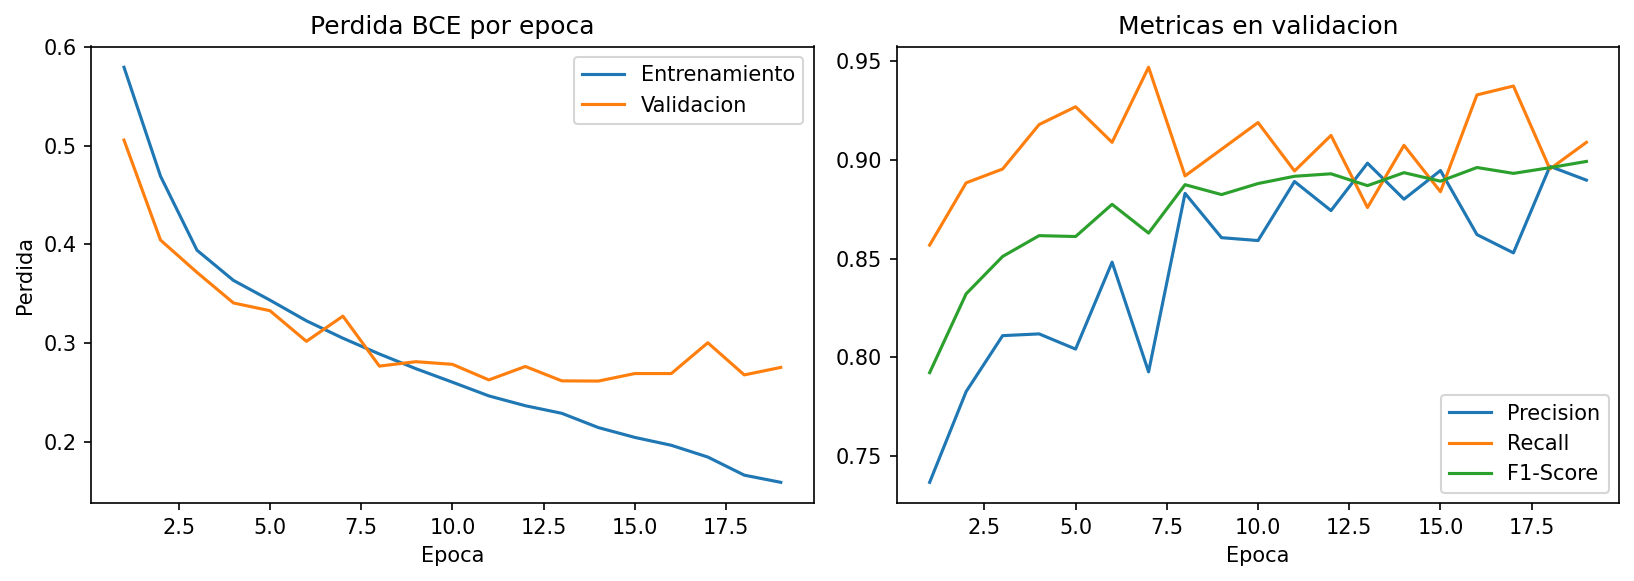
\includegraphics[width=0.98\linewidth]{curvas_entrenamiento.png}
  \caption{P\'erdida BCE (izq.) y m\'etricas de validaci\'on (der.) por \'epoca.
  La l\'inea vertical impl\'icita ocurre en la \'epoca 19, donde se activa la
  parada anticipada.}
  \label{fig:curvas}
\end{figure}

La Tabla~\ref{tab:evolucion} compara las m\'etricas en tres momentos clave del
entrenamiento para cuantificar el efecto de la estrategia de ajuste progresivo.
La Tabla~\ref{tab:prueba} reporta los resultados finales sobre el conjunto de
prueba.

\begin{table}[h]
\centering
\caption{Evoluci\'on de m\'etricas en validaci\'on por fase de entrenamiento.}
\label{tab:evolucion}
\resizebox{8.5cm}{!}{
\begin{tabular}{lccc}
\toprule
\textbf{Fase} & \textbf{Precisi\'on} & \textbf{Recall} & \textbf{F1} \\
\midrule
\'Ep. 3 --- embeddings congelados   & 0.811 & 0.895 & 0.851 \\
\'Ep. 6 --- inicio del ajuste fino  & 0.848 & 0.909 & 0.878 \\
\'Ep. 11 --- convergencia           & 0.889 & 0.894 & 0.892 \\
\'Ep. 19 --- parada anticipada      & 0.890 & 0.909 & 0.899 \\
\bottomrule
\end{tabular}}
\end{table}

\begin{table}[h]
\centering
\caption{M\'etricas finales en el conjunto de prueba (4\,000 muestras).}
\label{tab:prueba}
\begin{tabular}{lc}
\toprule
\textbf{M\'etrica} & \textbf{Valor} \\
\midrule
Precisi\'on  & 0.877 \\
Recall       & 0.910 \\
F1-Score     & \textbf{0.893} \\
\bottomrule
\end{tabular}
\end{table}

\subsection{Resultados cualitativos}

El recall supera sistem\'aticamente a la precisi\'on (0.910 frente a 0.877),
lo que indica una tendencia del modelo a clasificar como positivo ante la
ambig\"uedad. Esto es consistente con el sesgo de los vectores GloVe:
intensificadores frecuentes en rese\~nas como \textit{amazing} o
\textit{terrible} tienen carga emocional pronunciada que el modelo asocia con
la clase positiva incluso en contextos negativos. El efecto persiste tras el
ajuste fino.

La convergencia es r\'apida en las primeras seis \'epocas (F1: 0.792 a 0.878);
las \'epocas siguientes aportan mejoras marginales. La brecha creciente entre
p\'erdida de entrenamiento y validaci\'on a partir de la \'epoca 11 se\~nala
sobreajuste moderado que la parada anticipada contiene pero no elimina.

%%%%%%%%%%%%%%%%%%%%%%%%%%%%%%%%%%%%%%%%%%%%%%%%%%%%%%%%%%%%%%%%%%%%%%%%%%%%%%%%
\section{Discusi\'on}

El F1 de 0.893 es consistente con rangos reportados en trabajos sobre IMDb con
arquitecturas recurrentes \cite{howard2018}. El resultado se ubica en el rango
esperado para una sola capa LSTM, ya que \cite{greff2015} muestra que capas
adicionales no siempre mejoran el rendimiento y pueden introducir inestabilidad.

El mean pooling sobre los estados ocultos, respaldado por \cite{conneau2017},
produce representaciones m\'as estables que el \'ultimo estado oculto en
rese\~nas largas donde el sentimiento est\'a distribuido. La
Tabla~\ref{tab:evolucion} confirma que el ajuste fino de embeddings aporta 2.7
puntos de F1 entre las \'epocas 3 y 6, en l\'inea con \cite{kim2014} al
comparar embeddings est\'aticos y ajustables.

\textbf{Limitaciones:} el n\'umero de \'epocas de congelado es fijo; las
rese\~nas con m\'as de 300 tokens se truncan perdiendo el contexto final, y no
se realiz\'o b\'usqueda sistem\'atica de hiperpar\'ametros.

\textbf{Trabajo futuro:} comparar con un codificador Transformer ligero,
explorar mecanismos de atenci\'on como alternativa al mean pooling y evaluar
distintas duraciones de la fase de congelado.

%%%%%%%%%%%%%%%%%%%%%%%%%%%%%%%%%%%%%%%%%%%%%%%%%%%%%%%%%%%%%%%%%%%%%%%%%%%%%%%%
\clearpage

\begin{thebibliography}{99}

\bibitem{hochreiter1997}
S.~Hochreiter and J.~Schmidhuber,
``Long short-term memory,''
\textit{Neural Computation}, vol.~9, no.~8, pp.~1735--1780, 1997.

\bibitem{mikolov2013}
T.~Mikolov, K.~Chen, G.~Corrado, and J.~Dean,
``Efficient estimation of word representations in vector space,''
\textit{arXiv preprint arXiv:1301.3781}, 2013.

\bibitem{pennington2014}
J.~Pennington, R.~Socher, and C.~D.~Manning,
``GloVe: Global vectors for word representation,''
in \textit{Proc. EMNLP}, pp.~1532--1543, 2014.

\bibitem{maas2011}
A.~L.~Maas, R.~E.~Daly, P.~T.~Pham, D.~Huang, A.~Y.~Ng, and C.~Potts,
``Learning word vectors for sentiment analysis,''
in \textit{Proc. 49th Annual Meeting of the ACL}, pp.~142--150, 2011.

\bibitem{greff2015}
K.~Greff, R.~K.~Srivastava, J.~Kout\'nik, B.~R.~Steunebrink, and J.~Schmidhuber,
``LSTM: A search space odyssey,''
\textit{IEEE Trans. Neural Netw. Learn. Syst.}, vol.~28, no.~10,
pp.~2222--2232, 2017.

\bibitem{howard2018}
J.~Howard and S.~Ruder,
``Universal language model fine-tuning for text classification,''
in \textit{Proc. ACL}, pp.~328--339, 2018.

\bibitem{conneau2017}
A.~Conneau, D.~Kiela, H.~Schwenk, L.~Barrault, and A.~Bordes,
``Supervised learning of universal sentence representations from natural
language inference data,''
in \textit{Proc. EMNLP}, pp.~670--680, 2017.

\bibitem{kim2014}
Y.~Kim,
``Convolutional neural networks for sentence classification,''
in \textit{Proc. EMNLP}, pp.~1746--1751, 2014.

\bibitem{bird2009}
S.~Bird, E.~Klein, and E.~Loper,
\textit{Natural Language Processing with Python}.
O'Reilly Media, 2009.

\end{thebibliography}

\end{document}